\chapter{Methodology}
\label{example}
%In diesem Kapitel beschreiben Sie Ihren eigenen Beitrag
%- Es muss klar sein, worin die eigentliche Innovation besteht#

\section{Research Questions}
For this thesis we have selected 3 research questions. The first question : Can we use the visualization techniques to identify relevant properties of one performance-Influence model? The performance-influence models are of the format mentioned below:

\begin{equation*}
  \pi {(c)} = \overbrace{\underbrace {3}_{Coeff.} \cdot  \underbrace{{c(A)}}_{Option}}^{Term 1}  + \overbrace{ \underbrace{5}_{Coeff.} \cdot \underbrace{{c(B)}}_{Option}}^{Term 2} + \overbrace{\underbrace{0}_{Coeff.} \cdot \underbrace{{c(C)}}_{Option}}^{Term 3} - \overbrace{\underbrace{4}_{Coeff.} \cdot \underbrace{{ c(A)} \cdot {c(B)}}_{Interaction}}^{Term 4}
\end{equation*}

The set of valid performance-influence models are put into a csv file. And these csv files are used as an input for the visualization. 

From the visualizations we can identify the data point that is either the highest or lowest point that influences the systems performance the most.

Second research question : Can we use the visualization to compare two performance-influence models?. Many times a version of a software needs to be compared to its next version to check how the two versions differ in terms of its performance. In this case, we have two performance-influence models in one csv file, and use this as an input to the visualization. hence comparison of two different performance-influence models can be done, and identify if the same configuration option causes a spike in performance in either of the versions.

Third research question : How do the visualizations scale?. when a configurable software has added new configuration options, new performance-influence models are derived to reflect its performance influence over the system. The new performance-influence models are then used as an input to the visualization. Scaling can be of two types. One, addition of new configuration option. Two, addition of new performance-influence model to the same csv file. Both of the types of scaling are implemented in the thesis.

\section{Why the above Research Questions?}
The research questions are selected based on number of performance-influence models we visualize at the same time. When we have only one performance-influence model, we would like to know the configuration option that has affected the performance the highest, it can be maximum performance increase or decrease. 

when we look at the two performance-influence models, we are basically comparing the two and finding out the configuration that either differs the most or is the most similar. The configuration option that differs the most can indicate that this configuration option has caused a performance spike in one of the versions, it can be positive or negative spike. The configuration option that have been the most similar indicate that in the second version of the software, this configuration option remained unaffected.

when we look at more than 2 performance-influence models, we have comparing several versions of the same software with increasing configuration options in each versions. This visualization helps to see what would be the outliers, or which set of performance-influence models have share similar set of influences.


\section{Acronyms}

This template makes advantage of the glossaries package to support acronyms. The first occurence of an acronym is replaced by its definition (e.g., \gls{IDE}). All other occurences are replaced by the acronym (\gls{IDE}). The glossaries package also supports plural---\glspl{IDE}.

\glsreset{IDE}
Sometimes you want to make sure, that the long version is used, even if \gls{IDE} was inserted before.
 
\section{Citation}

There are several types of literature. The most citations are workshop and conference papers. Please use the inproceedings-tag for those citations (e.g., \cite{KAK:GPCE09}). You should have short-hands for workshop and conference names to be sure the naming is consistent and uniform (see our BibTeX files how to do that).
 
Slightly different are articles published in journals (e.g., \cite{KG:SME06}). Make sure you that the volume and number-tags are present and that no inproceeding is tagged as article or vice versa.

You might want to take a look at the example BibTeX file to find out how to cite books~\cite{CE:BOOK00}, technical reports~\cite{KCHNP:TR90}, websites~\cite{Coq:website}, PhD theses, or master theses~\cite{B:PHD03,R:MT09}.

\section{Formulas}
 
There are different types of mathematical environments to set formulas. The equation $E=m\cdot c^2$ is an inline formula. But you can also have formulas at a separate line (see \vref{eq:ex}).

	\begin{equation}\label{eq:ex}
			P=\bigl(\mathcal{A}\pimplies(\mathcal{B}\pequals\mathcal{C})\pand(\mathcal{B}\pequals\mathcal{D})\bigr)\pand(\mathcal{B}\pimplies\mathcal{A})\pand(\mathcal{C}\pimplies\mathcal{A})\pand(\mathcal{D}\pimplies\mathcal{A})
	\end{equation}

If you need multiple lines that are aligned to each other, you might want to use the following code.

	\newcommand{\fG}{\mbox{GraphLibrary}}
	\newcommand{\fE}{\mbox{Edges}}
	\newcommand{\fA}{\mbox{Algorithms}}
	\newcommand{\fD}{\mbox{Directed}}
	\newcommand{\fU}{\mbox{Undirected}}
	\newcommand{\fN}{\mbox{Number}}
	\newcommand{\fC}{\mbox{Cycle}}
	\begin{eqnarray*}
	&& \fG\\
	&\pand& (\fG \pimplies \fE) \pand (\fE \por \fA \pimplies \fG)\\
	&\pand& (\fE \pequals \fD \por \fU) \pand (\pnot \fD \por \pnot \fU)\\
	&\pand& (\fA \pequals \fN \por \fC)\\
	&\pand& (\fC \pimplies \fD).\\
	\end{eqnarray*}

\section{Graphics}

In \vref{fig:ex}, we give a small example how to insert and reference a figure.

\begin{figure}[htbp]
	\centering
		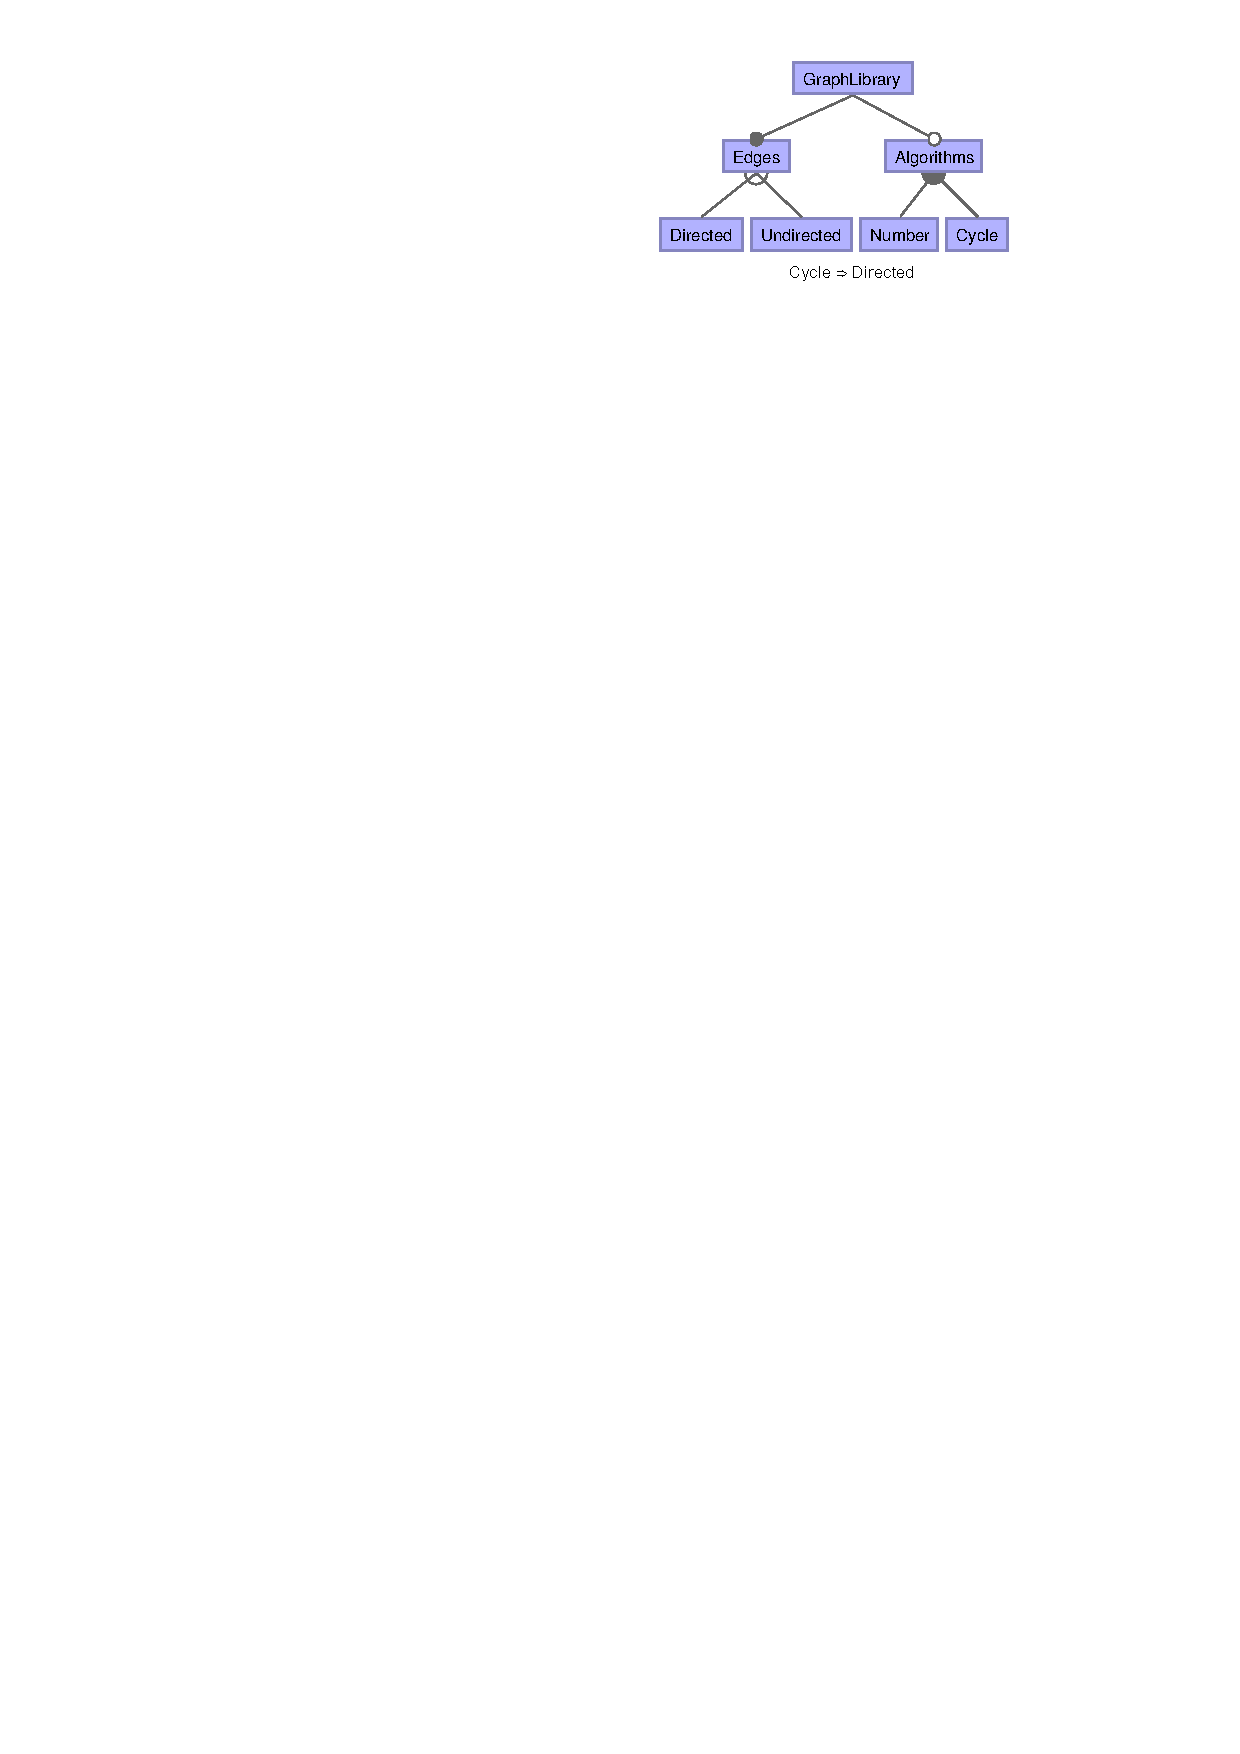
\includegraphics[scale=1.25]{example}
	\caption{A feature model representing a graph product line}
	\label{fig:ex}
\end{figure}

\section{Tables}

\vref{tab:ex} shows the result of a simple tabular environment.

\begin{table}[htbp]
	\centering
		\begin{tabular}{cc}\toprule
			Group Type & Propositional Formula\\\midrule
			And & $(P \pimplies C_{k_1} \wedge\ldots\wedge C_{k_m}) \pand (C_1\vee\ldots\vee C_n \pimplies P)$\\\addlinespace
			Or & $P \pequals C_1\vee\ldots\vee C_n$\\\addlinespace
			Alternative & $(P \pequals C_1\vee\ldots\vee C_n) \pand \mbox{atmost}1(C_1,\ldots,C_n)$\\
			\bottomrule
		\end{tabular}
	\caption{Mapping a feature model to a propositional formula}
	\label{tab:ex}
\end{table}

\section{Code Listings}

In \vref{lst:ex}, we give an example of a source code listing. 

\begin{lstlisting}[style=Java,float=htb,caption={Java source code},label={lst:ex}]
class A extends Object {
	A() { super(); }
}
class B extends Object {
	B() { super(); }
}
class Pair extends Object {
	Object fst;
	Object snd;
	Pair(Object fst, Object snd) {
		super(); this.fst=fst; this.snd=snd;
	}
	Pair setfst(Object newfst) {
		return new Pair(newfst, this.snd);
	}
}
\end{lstlisting}
